\subsection{多线程优化}

CBC模式不能利用并行计算加速不同明文分组的处理过程,因为加密计算过程:
\[   C_{i+1} = Enc_k(C_i \oplus m_{i+1})    \]
可以看到,加密第$i+1$个明文分组的过程需要第$i$个密文分组参与,而计算第$i$个密文分组又需要第$i-1$个密文分组参与,因此只能
逐分组加密。因此,本实验没有把单条CBC消息的加密过程错误地拆成分组并行,而是采用多缓冲区并行策略:每个线程处理一条独立的CBC数据流,各数据流使用独立IV并各自保持内部串行依赖。该方法对应实际系统中同时处理多个加密请求的场景,属于SM4-CBC工程实现层面的吞吐量优化。
对应代码编译运行后结果如下图\footnote{更多测试案例和对应结果见实验结果章节}:
\begin{figure}[H]
    \centering
    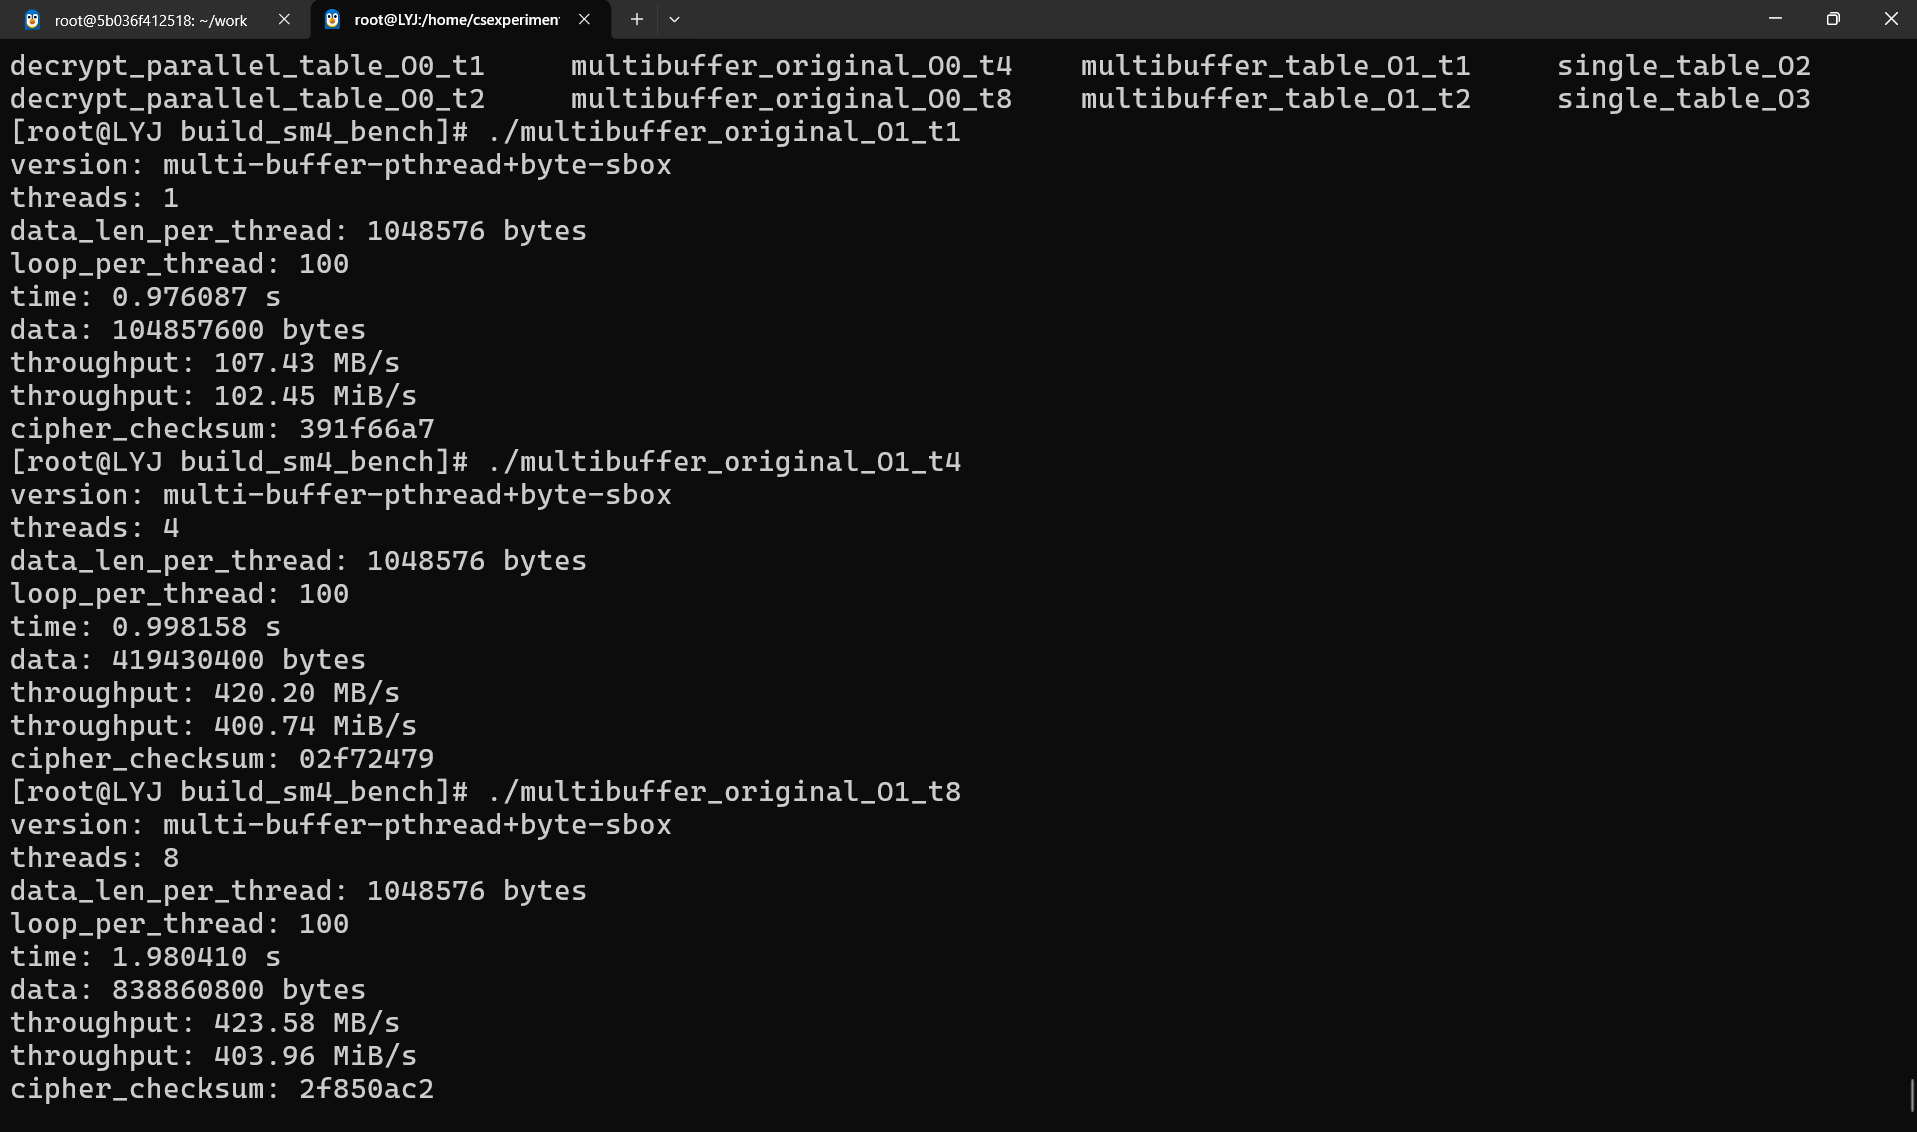
\includegraphics[width = 1\textwidth]{figure/parallel_encrypt_without_table.png}
    \caption{主机多线程优化加密(-O1)}
\end{figure}

由CBC模式原理可知,解密阶段所有密文分组在开始时已经可见,因此每个分组的\(D(C_i)\)可以并行计算,再与\(C_{i-1}\)或IV异或得到明文。本实验据此实现SM4-CBC并行解密算法,编译运行结果如下图:
\begin{figure}[H]
    \centering
    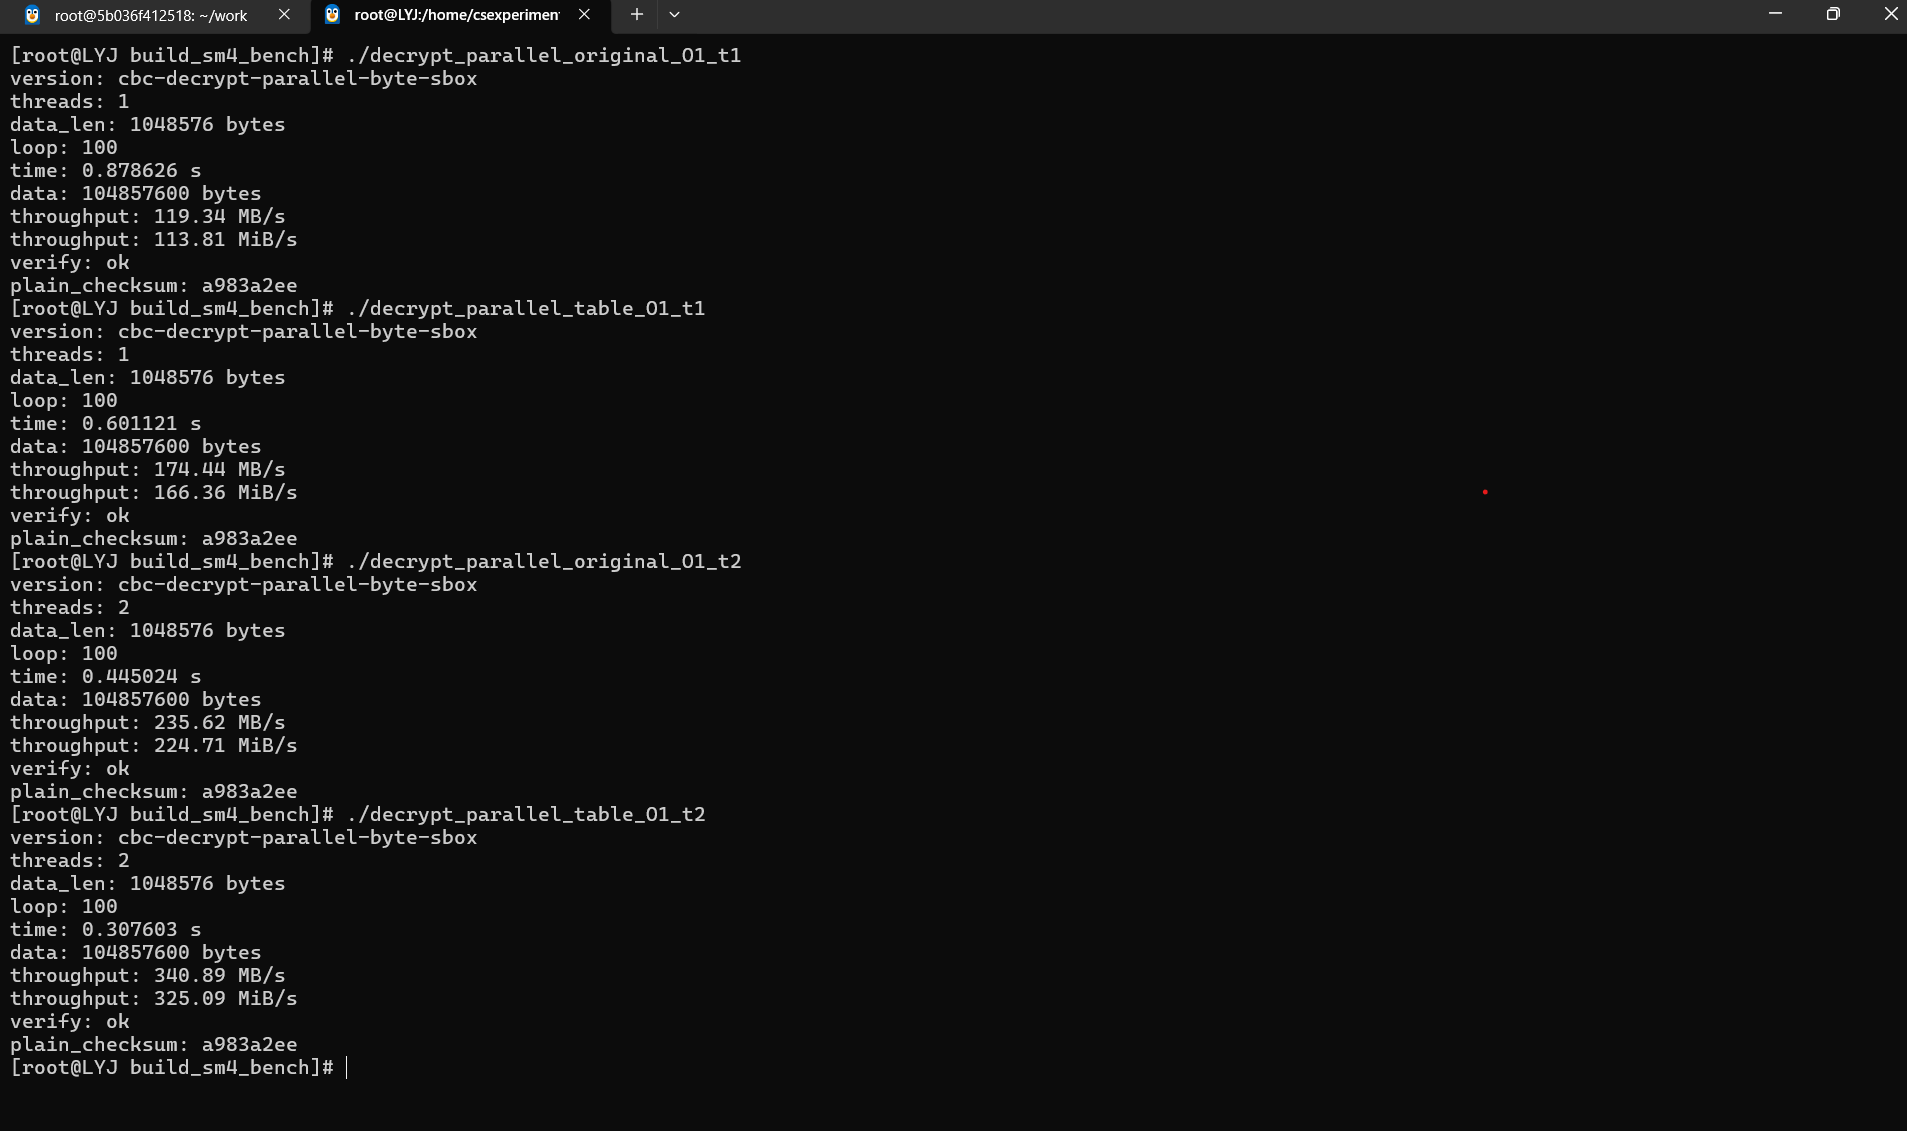
\includegraphics[width = 1\textwidth]{figure/parallel_decrypt.png}
    \caption{主机多线程并行优化解密}
\end{figure}


将上述优化转移至QEMU模拟器中的RISC-V架构上实现。宿主机侧使用RISC-V GNU工具链进行静态交叉编译,将可执行文件和批量运行脚本复制到根文件系统镜像的\verb|/tmp|目录,随后启动QEMU运行RISC-V Linux。启动过程如下图:
\begin{figure}[H]
    \centering
    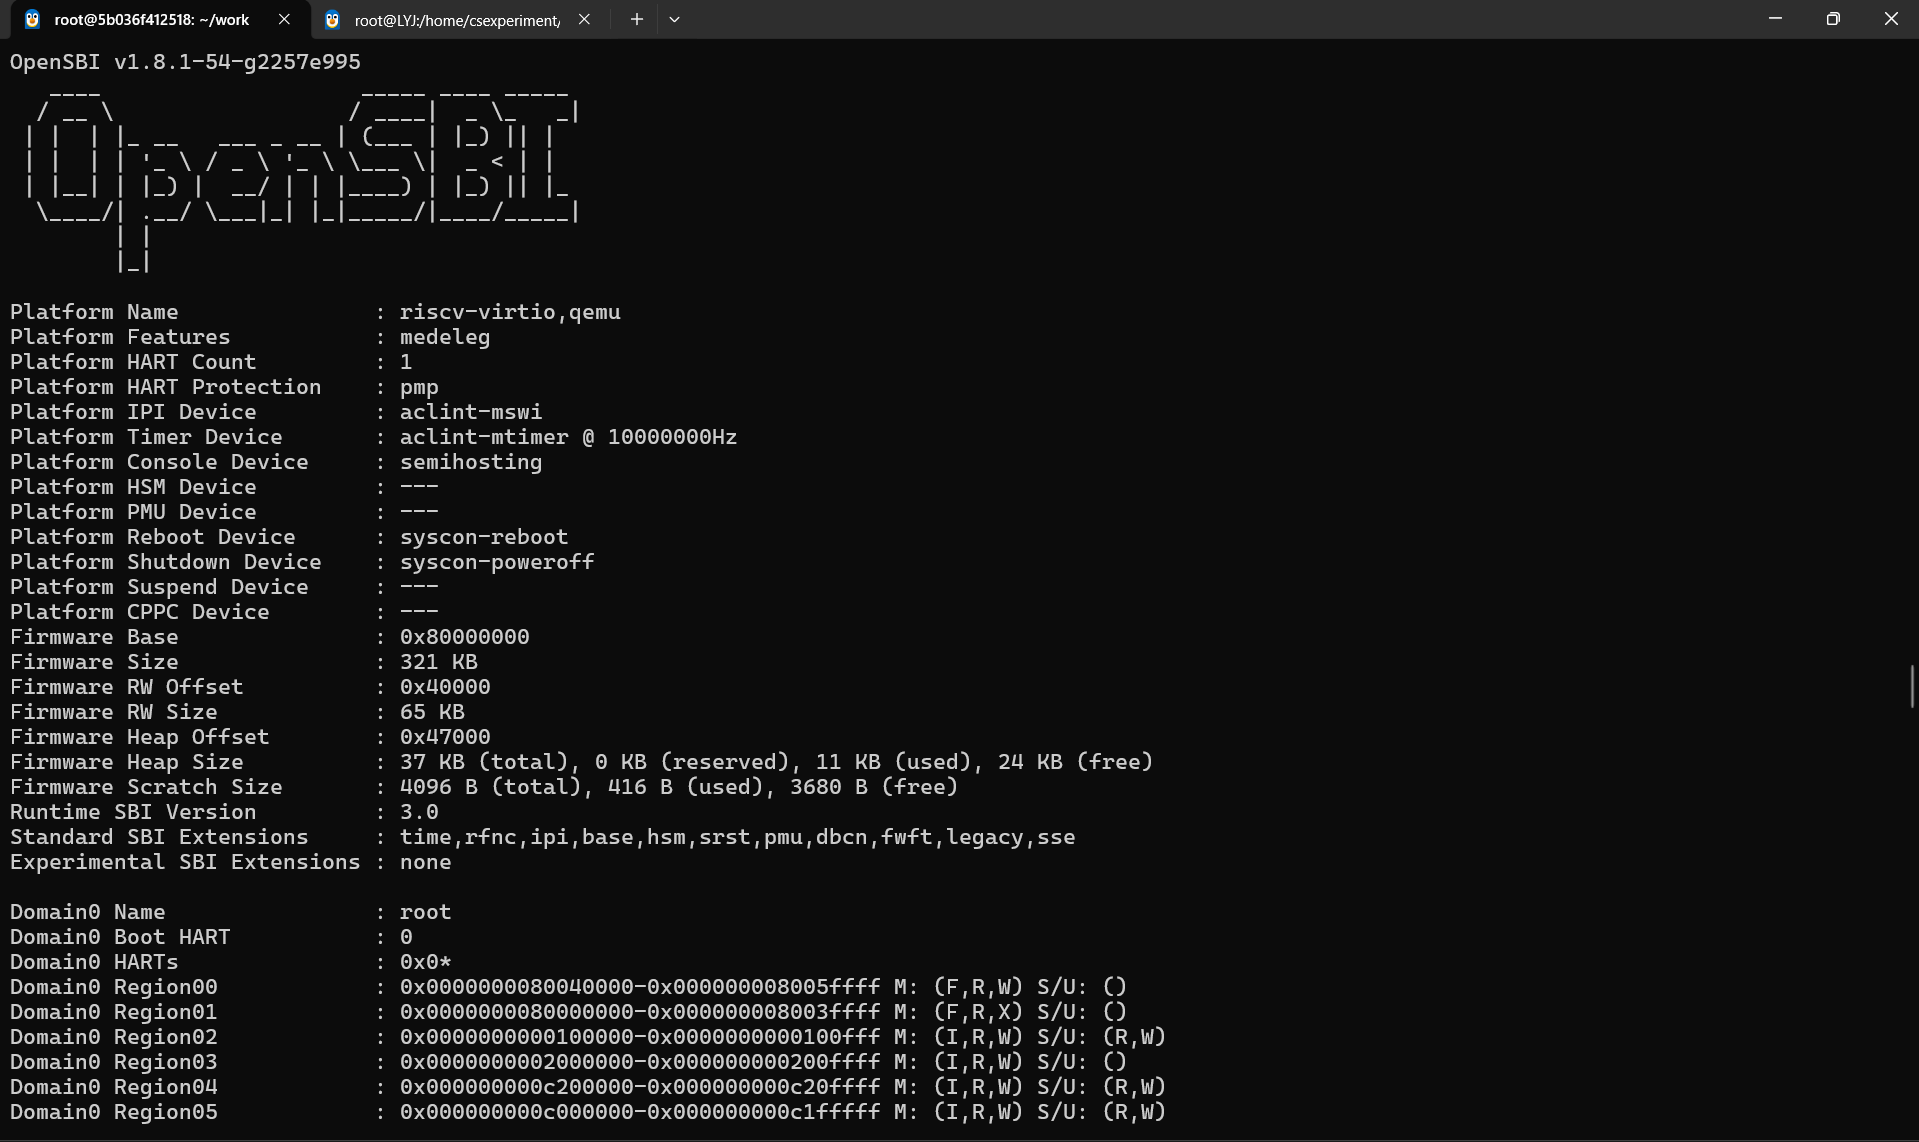
\includegraphics[width = 1\textwidth]{figure/OpenSBI.png}
    \caption{启动qemu模拟器}
\end{figure}
相同并行优化代码运行结果分别如下图:
\begin{figure}[H]
    \centering
    \begin{subfigure}[并行加密优化]{
        \begin{minipage}[b]{1 \textwidth}
            \centering
        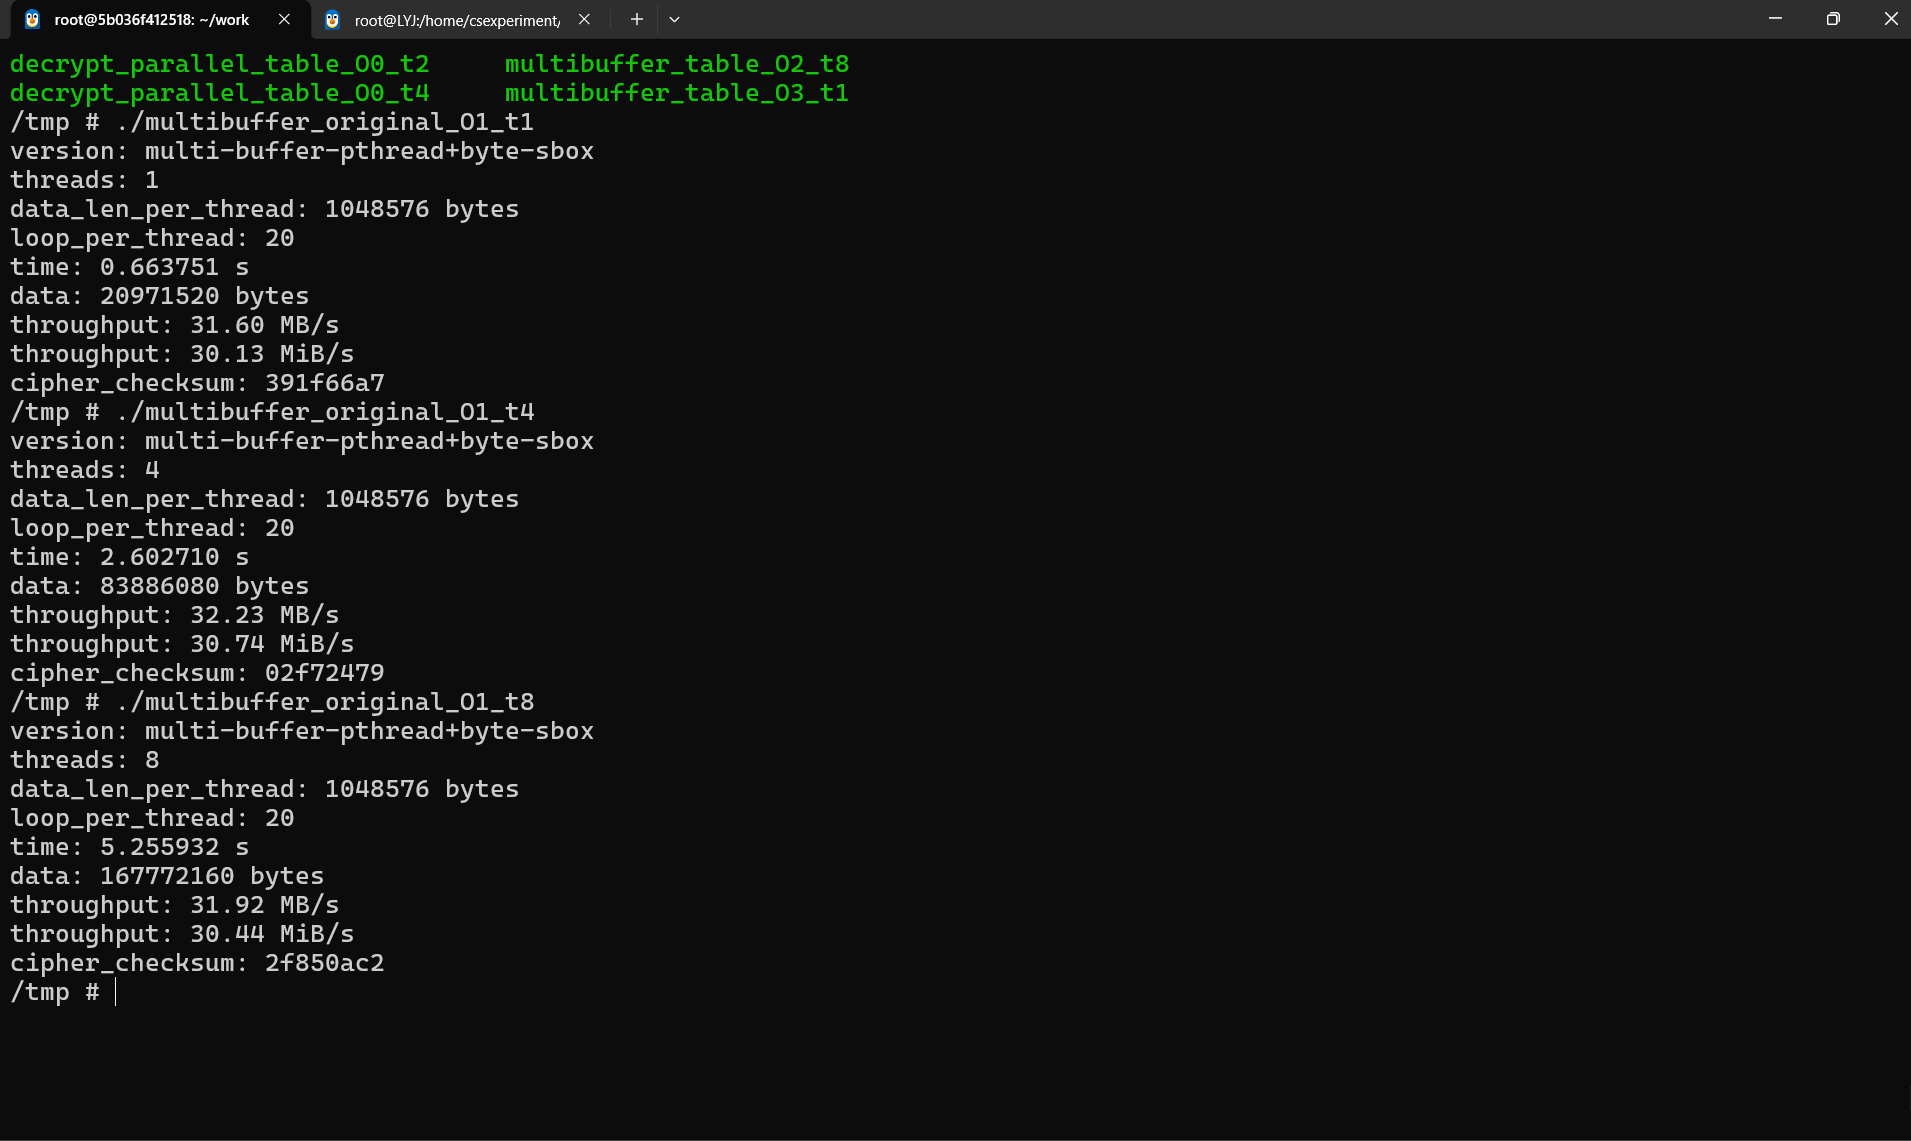
\includegraphics[width = 1\textwidth]{figure/parallel_encrypt_qemu.png}
        \end{minipage}
        }
    \end{subfigure}
    \begin{subfigure}[并行解密优化]{
        \begin{minipage}[b]{1 \textwidth}
            \centering
        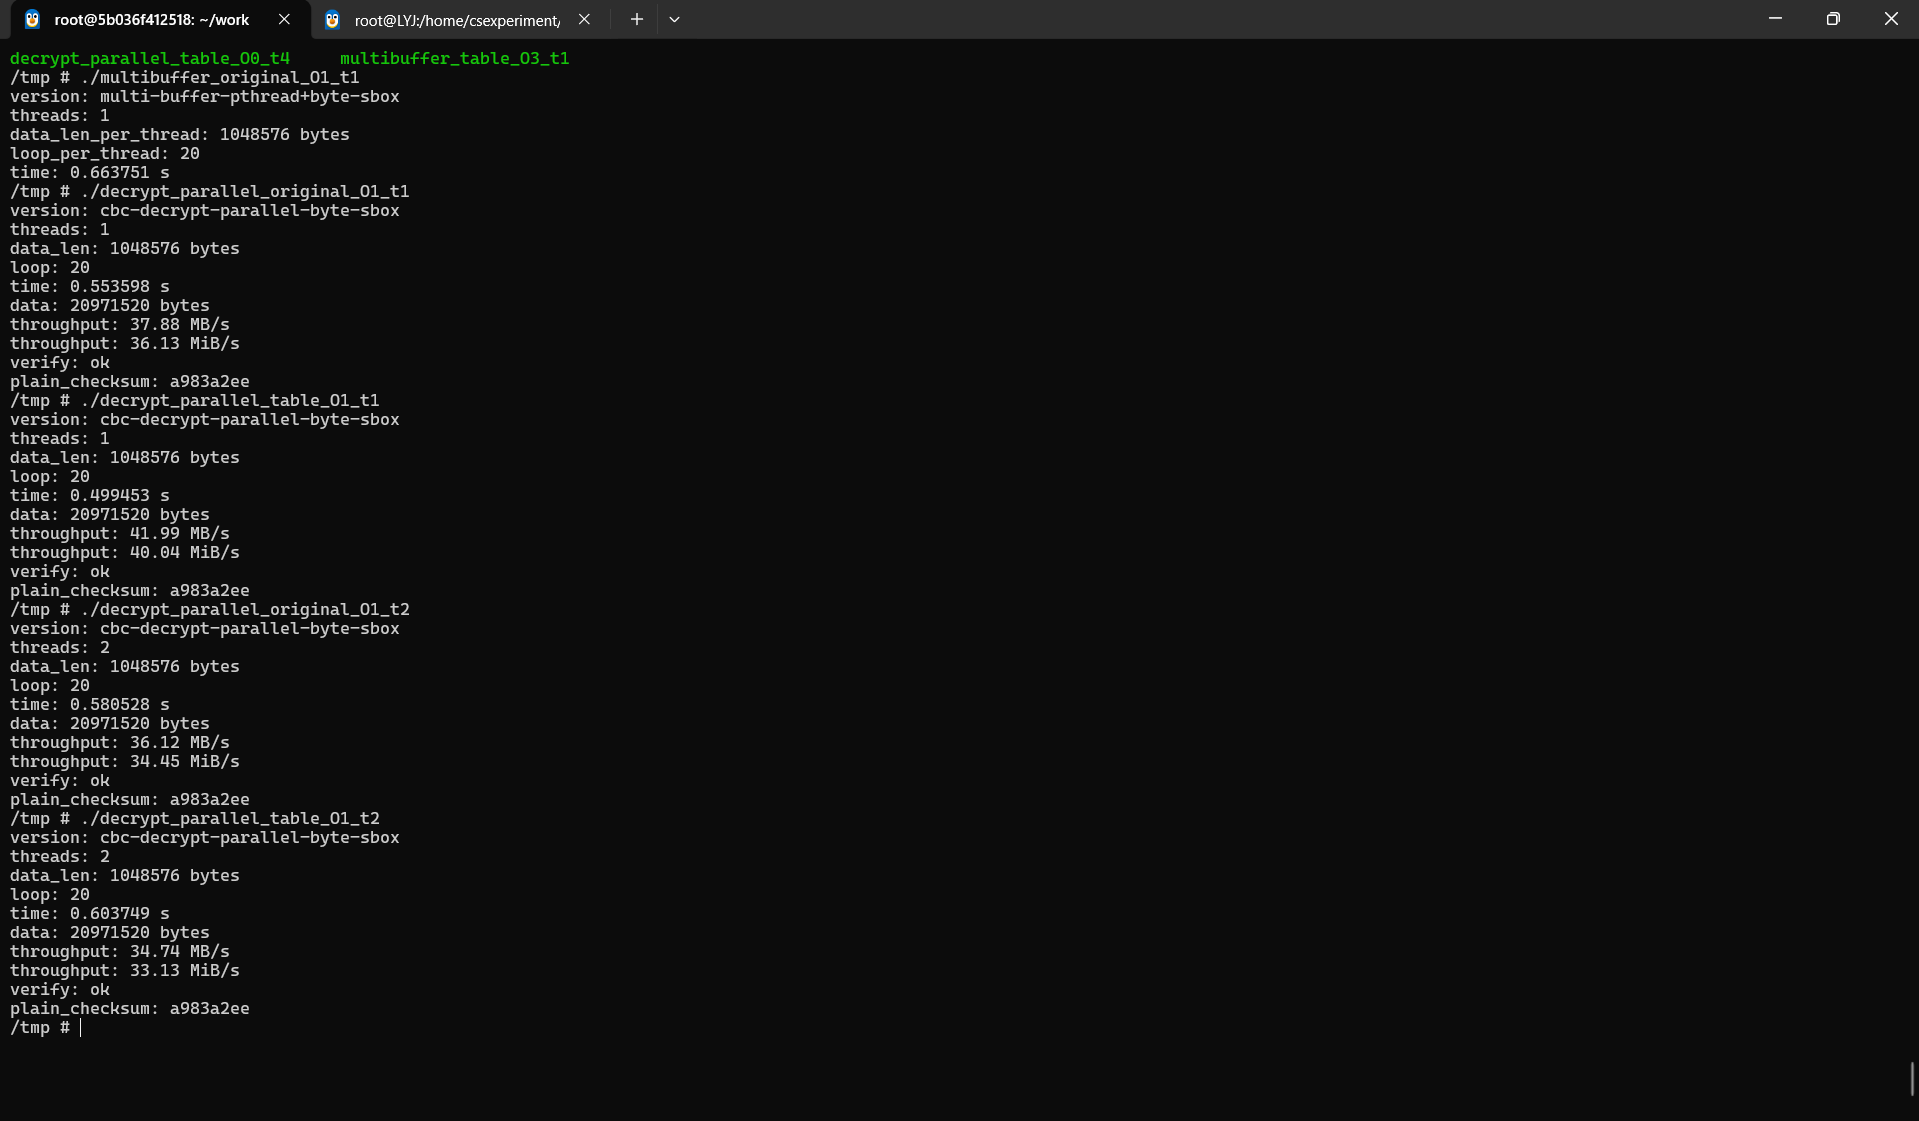
\includegraphics[width =  1\textwidth]{figure/parallel_decrypt_qemu.png}
        \end{minipage}
        }
    \end{subfigure}
    \caption{qemu模拟器上运行优化代码结果}
\end{figure}



